\documentclass[11pt,a4paper]{report}
\usepackage[textwidth=37em,vmargin=30mm]{geometry}
\usepackage{calc,xunicode,amsmath,amssymb,paralist,enumitem,tabu,booktabs,datetime2,xeCJK,xeCJKfntef,listings}
\usepackage{tocloft,fancyhdr,tcolorbox,xcolor,graphicx,eso-pic,xltxtra,xelatexemoji}

\newcommand{\envyear}[0]{2025}
\newcommand{\envdatestr}[0]{2025-07-30}
\newcommand{\envfinaldir}[0]{webdb/2025/20250730/final}

\usepackage[hidelinks]{hyperref}
\hypersetup{
    colorlinks=false,
    pdfpagemode=FullScreen,
    pdftitle={Web Digest - \envdatestr}
}

\setlength{\cftbeforechapskip}{10pt}
\renewcommand{\cftchapfont}{\rmfamily\bfseries\large\raggedright}
\setlength{\cftbeforesecskip}{2pt}
\renewcommand{\cftsecfont}{\sffamily\small\raggedright}

\setdefaultleftmargin{2em}{2em}{1em}{1em}{1em}{1em}

\usepackage{xeCJK,xeCJKfntef}
\xeCJKsetup{PunctStyle=plain,RubberPunctSkip=false,CJKglue=\strut\hskip 0pt plus 0.1em minus 0.05em,CJKecglue=\strut\hskip 0.22em plus 0.2em}
\XeTeXlinebreaklocale "zh"
\XeTeXlinebreakskip = 0pt


\setmainfont{Brygada 1918}
\setromanfont{Brygada 1918}
\setsansfont{IBM Plex Sans}
\setmonofont{JetBrains Mono NL}
\setCJKmainfont{Noto Serif CJK SC}
\setCJKromanfont{Noto Serif CJK SC}
\setCJKsansfont{Noto Sans CJK SC}
\setCJKmonofont{Noto Sans CJK SC}

\setlength{\parindent}{0pt}
\setlength{\parskip}{8pt}
\linespread{1.15}

\lstset{
	basicstyle=\ttfamily\footnotesize,
	numbersep=5pt,
	backgroundcolor=\color{black!5},
	showspaces=false,
	showstringspaces=false,
	showtabs=false,
	tabsize=2,
	captionpos=b,
	breaklines=true,
	breakatwhitespace=true,
	breakautoindent=true,
	linewidth=\textwidth
}






\newcommand{\coverpic}[2]{
    % argv: itemurl, authorname
    Cover photo by #2~~(\href{#1}{#1})
}
\newcommand{\makeheader}[0]{
    \begin{titlepage}
        % \newgeometry{hmargin=15mm,tmargin=21mm,bmargin=12mm}
        \begin{center}
            
            \rmfamily\scshape
            \fontspec{BaskervilleF}
            \fontspec{Old Standard}
            \fontsize{59pt}{70pt}\selectfont
            WEB\hfill DIGEST
            
            \vfill
            % \vskip 30pt
            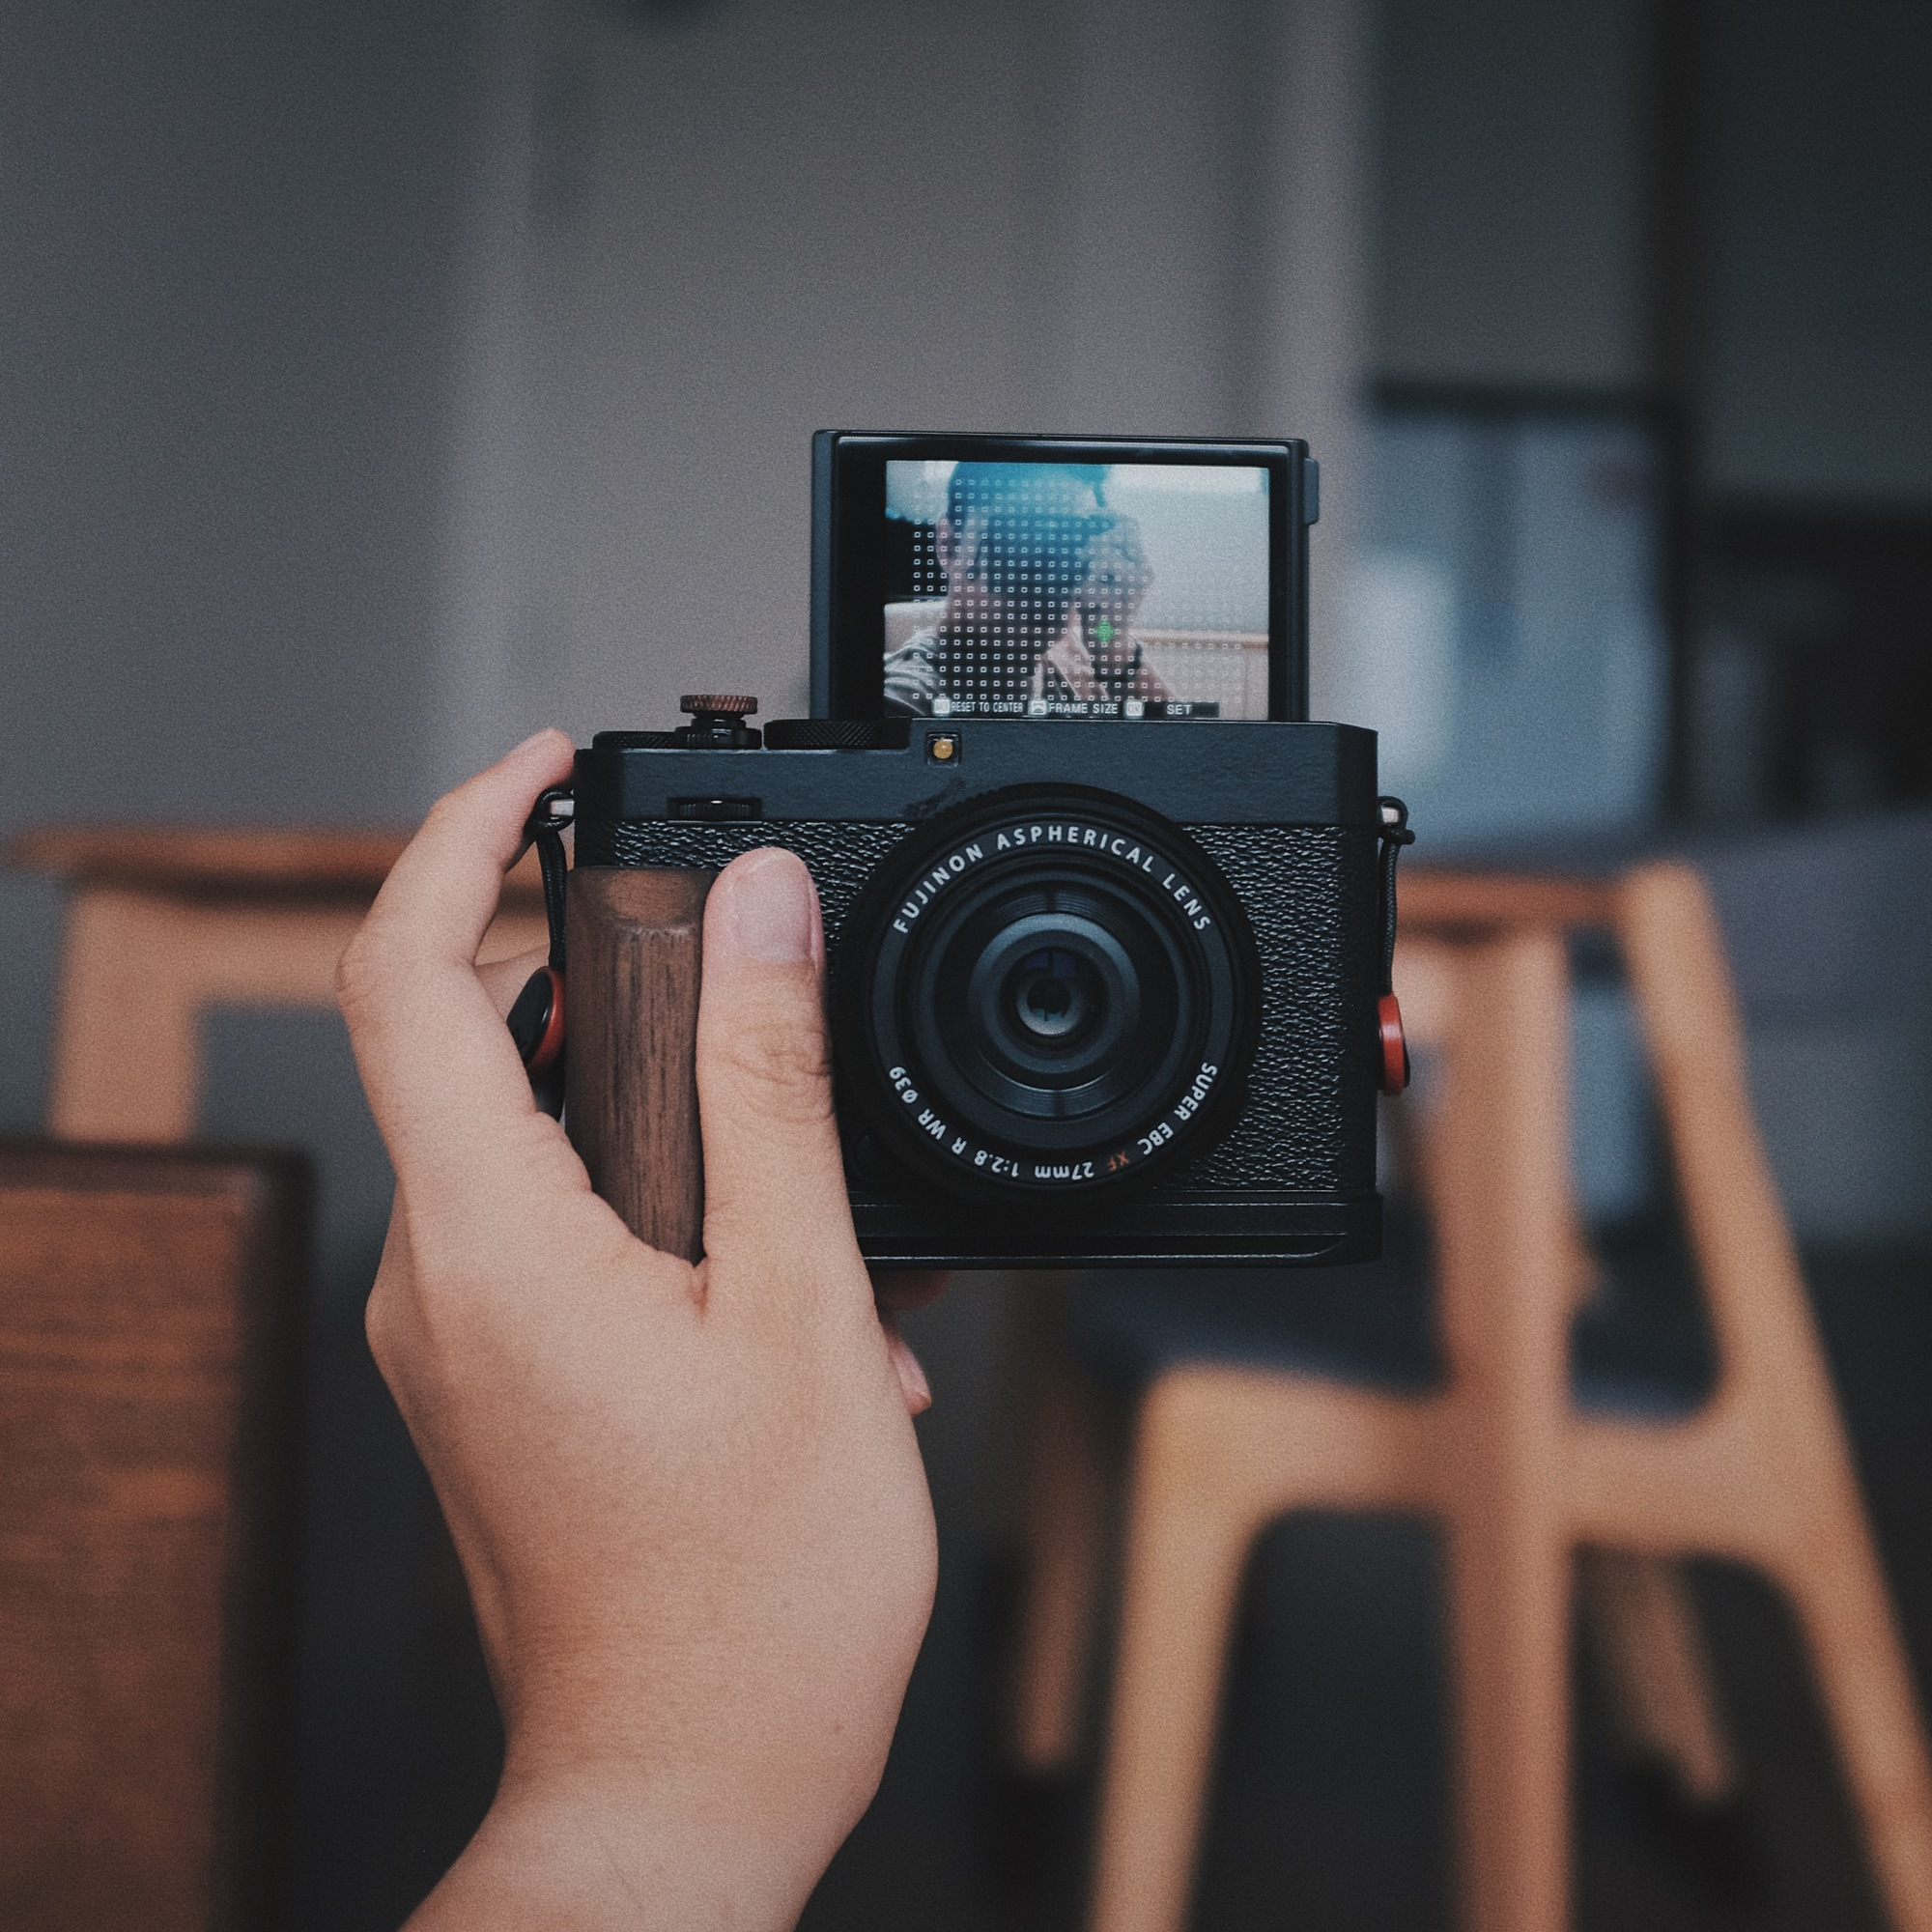
\includegraphics[width=\linewidth]{\envfinaldir/coverpic-prod.jpg}\par
            % \vskip 30pt
            \vfill

            \normalsize\rmfamily\scshape
            \copyright{} The Web Digest Project \hfill\large \envdatestr
        \end{center}
    \end{titlepage}
    % \restoregeometry
}
\newcommand{\simplehref}[1]{%
    \textcolor{blue!80!green}{\href{#1}{#1}}%
}
\renewcommand{\contentsname}{\center\Huge\sffamily\bfseries Contents\par\vskip 20pt}
\newcounter{ipartcounter}
\setcounter{ipartcounter}{0}
\newcommand{\ipart}[1]{
    % \vskip 20pt
    \clearpage
    \stepcounter{ipartcounter}
    \phantomsection
    \addcontentsline{toc}{chapter}{#1}
    % \begin{center}
    %     \Huge
    %     \sffamily\bfseries
    %     #1
    % \end{center}
    % \vskip 20pt plus 7pt
}
\newcounter{ichaptercounter}
\setcounter{ichaptercounter}{0}
\newcommand{\ichapter}[1]{
    % \vskip 20pt
    \clearpage
    \stepcounter{ichaptercounter}
    \phantomsection
    \addcontentsline{toc}{section}{\numberline{\arabic{ichaptercounter}}#1}
    \begin{center}
        \Huge
        \sffamily\bfseries
        #1
    \end{center}
    \vskip 20pt plus 7pt
}
\newcommand{\entrytitlefont}[1]{\subsection*{\raggedright\Large\sffamily\bfseries#1}}
\newcommand{\entryitemGeneric}[2]{
    % argv: title, url
    \parbox{\linewidth}{
        \entrytitlefont{#1}\par\vskip 5pt
        \footnotesize\ttfamily\mdseries
        \simplehref{#2}
    }\vskip 11pt plus 11pt minus 1pt
}
\newcommand{\entryitemGithub}[3]{
    % argv: title, url, desc
    \parbox{\linewidth}{
        \entrytitlefont{#1}\par\vskip 5pt
        \footnotesize\ttfamily\mdseries
        \simplehref{#2}\par\vskip 5pt
        \small\rmfamily\mdseries#3
    }\vskip 11pt plus 11pt minus 1pt
}
\newcommand{\entryitemAp}[3]{
    % argv: title, url, desc
    \parbox{\linewidth}{
        \entrytitlefont{#1}\par\vskip 5pt
        \footnotesize\ttfamily\mdseries
        \simplehref{#2}\par\vskip 5pt
        \small\rmfamily\mdseries#3
    }\vskip 11pt plus 11pt minus 1pt
}
\newcommand{\entryitemHackernews}[3]{
    % argv: title, hnurl, rawurl
    % \parbox{\linewidth}{
    %     \entrytitlefont{#1}\par\vskip 5pt
    %     \footnotesize\ttfamily\mdseries
    %     \simplehref{#3}\par
    %     \textcolor{black!50}{\href{#2}{#2}}
    % }\vskip 11pt plus 11pt minus 1pt
    \begin{minipage}{\linewidth}
            \entrytitlefont{#1}\par\vskip 5pt
            \footnotesize\ttfamily\mdseries
            \simplehref{#3}\par
            \textcolor{black!50}{\href{#2}{#2}}
    \end{minipage}\par\vskip 11pt plus 11pt minus 1pt
}







\begin{document}

\makeheader

\tableofcontents\clearpage




\ipart{Developers}
\ichapter{Hacker News}
\entryitemTwoLinks{Webflow Down for >31 Hours}{https://news.ycombinator.com/item?id=44728554}{https://status.webflow.com}

\entryitemTwoLinks{Microsoft bans LibreOffice developer's account without warning, rejects appeal}{https://news.ycombinator.com/item?id=44728369}{https://www.neowin.net/news/microsoft-bans-libreoffice-developers-account-without-warning-rejects-appeal/}

\entryitemTwoLinks{More honey bees dying, even as antibiotic use halves}{https://news.ycombinator.com/item?id=44727420}{https://news.uoguelph.ca/2025/07/more-honey-bees-dying-even-as-antibiotic-use-halves/}

\entryitemTwoLinks{Maru OS – Use your phone as your PC}{https://news.ycombinator.com/item?id=44727298}{https://maruos.com/}

\entryitemTwoLinks{Linux 6.16: faster file systems, improved confidential memory, more Rust support}{https://news.ycombinator.com/item?id=44726551}{https://www.zdnet.com/article/linux-6-16-brings-faster-file-systems-improved-confidential-memory-support-and-more-rust-support/}

\entryitemTwoLinks{Study mode}{https://news.ycombinator.com/item?id=44725764}{https://openai.com/index/chatgpt-study-mode/}

\entryitemTwoLinks{Learning basic electronics by building fireflies}{https://news.ycombinator.com/item?id=44725757}{http://a64.in/posts/learning-basic-electronics-by-building-fireflies/}

\entryitemTwoLinks{Launch HN: Hyprnote (YC S25) – An open-source AI meeting notetaker}{https://news.ycombinator.com/item?id=44725306}{https://news.ycombinator.com/item?id=44725306}

\entryitemTwoLinks{Show HN: I built an AI that turns any book into a text adventure game}{https://news.ycombinator.com/item?id=44725202}{https://www.kathaaverse.com/}

\entryitemTwoLinks{Irrelevant facts about cats added to math problems increase LLM errors by 300\%}{https://news.ycombinator.com/item?id=44724238}{https://www.science.org/content/article/scienceadviser-cats-confuse-ai}

\entryitemTwoLinks{Observable Notebooks 2.0 Technology Preview}{https://news.ycombinator.com/item?id=44724068}{https://observablehq.com/notebook-kit/}

\entryitemTwoLinks{Learning Is Slower Than You Think}{https://news.ycombinator.com/item?id=44723763}{https://nisheethvishnoi.substack.com/p/learning-is-slower-than-you-think}

\entryitemTwoLinks{My 2.5 year old laptop can write Space Invaders in JavaScript now (GLM-4.5 Air)}{https://news.ycombinator.com/item?id=44723316}{https://simonwillison.net/2025/Jul/29/space-invaders/}

\entryitemTwoLinks{Linux Performance Analysis (2015)}{https://news.ycombinator.com/item?id=44722951}{https://netflixtechblog.com/linux-performance-analysis-in-60-000-milliseconds-accc10403c55}

\entryitemTwoLinks{Show HN: Terminal-Bench-RL: Training Long-Horizon Terminal Agents with RL}{https://news.ycombinator.com/item?id=44721791}{https://github.com/Danau5tin/terminal-bench-rl}

\entryitemTwoLinks{UK Online Safety Act sends VPN use soaring}{https://news.ycombinator.com/item?id=44721772}{https://www.wired.com/story/vpn-use-spike-age-verification-laws-uk/}

\entryitemTwoLinks{Wikimedia Foundation Challenges UK Online Safety Act Regulations}{https://news.ycombinator.com/item?id=44721403}{https://wikimediafoundation.org/news/2025/07/17/wikimedia-foundation-challenges-uk-online-safety-act-regulations/}

\entryitemTwoLinks{Nothing to watch – Experimental gallery visualizing 50k film posters}{https://news.ycombinator.com/item?id=44721204}{https://nothing-to-watch.port80.ch}

\entryitemTwoLinks{Stop selling ``unlimited'', when you mean ``until we change our minds''}{https://news.ycombinator.com/item?id=44721003}{https://blog.kilocode.ai/p/ai-pricing-playbook-strikes-again}

\entryitemTwoLinks{The EU could be scanning your chats by October 2025}{https://news.ycombinator.com/item?id=44720103}{https://www.techradar.com/computing/cyber-security/the-eu-could-be-scanning-your-chats-by-october-2025-heres-everything-we-know}


\ipart{Developers~~~~(zh-Hans)}
\ichapter{Solidot}
\entryitemGeneric{\hskip 0pt{}经济学家称挪威人太富裕且太舒坦了}{https://www.solidot.org/story?sid=81919}

\entryitemGeneric{\hskip 0pt{}中国大学鼓励学生使用 AI}{https://www.solidot.org/story?sid=81918}

\entryitemGeneric{\hskip 0pt{}未成年人参与了秦兵马俑的制作}{https://www.solidot.org/story?sid=81917}

\entryitemGeneric{\hskip 0pt{}北京火狐从 9 月 29 日起不再运营 Firefox 在华业务}{https://www.solidot.org/story?sid=81916}

\entryitemGeneric{\hskip 0pt{}银河系发现首个幽灵行星状星云}{https://www.solidot.org/story?sid=81915}

\entryitemGeneric{\hskip 0pt{}教育能否延缓认知衰退?}{https://www.solidot.org/story?sid=81914}

\entryitemGeneric{\hskip 0pt{}安全研究员发现 SkyRover X1 是更换品牌的大疆产品}{https://www.solidot.org/story?sid=81913}

\entryitemGeneric{\hskip 0pt{}人类组织蛋白质在 50 岁左右加速衰老}{https://www.solidot.org/story?sid=81912}

\entryitemGeneric{\hskip 0pt{}三星 One UI 8 禁止解锁 bootloader}{https://www.solidot.org/story?sid=81911}

\entryitemGeneric{\hskip 0pt{}索尼指控腾讯抄袭其《地平线》系列游戏}{https://www.solidot.org/story?sid=81910}

\entryitemGeneric{\hskip 0pt{}在 Online Safety Act 生效后英国 VPN 使用量激增}{https://www.solidot.org/story?sid=81909}

\entryitemGeneric{\hskip 0pt{}挪威开始在海底储存液化二氧化碳}{https://www.solidot.org/story?sid=81908}

\entryitemGeneric{\hskip 0pt{}FFmpeg 8.0 预计八月底释出}{https://www.solidot.org/story?sid=81907}

\entryitemGeneric{\hskip 0pt{}腾讯发布混元世界 1.0 模型}{https://www.solidot.org/story?sid=81906}

\entryitemGeneric{\hskip 0pt{}针对开源软件的供应链攻击失控}{https://www.solidot.org/story?sid=81905}

\entryitemGeneric{\hskip 0pt{}英特尔终止 PlaidML 开源深度学习软件开发}{https://www.solidot.org/story?sid=81904}

\entryitemGeneric{\hskip 0pt{}Linux 6.16 释出}{https://www.solidot.org/story?sid=81903}

\entryitemGeneric{\hskip 0pt{}ChatGPT 让我们变蠢?}{https://www.solidot.org/story?sid=81902}

\entryitemGeneric{\hskip 0pt{}Stack Exchange 迁移到云端}{https://www.solidot.org/story?sid=81901}

\entryitemGeneric{\hskip 0pt{}今天的环法自行车选手已经超越了当年的阿姆斯特朗}{https://www.solidot.org/story?sid=81900}\ichapter{V2EX}
\entryitemGeneric{\hskip 0pt{}[问与答] 有没有哪家共享电动车可以买月卡的?}{https://www.v2ex.com/t/1148627}

\entryitemGeneric{\hskip 0pt{}[Solana] 用 \$V2EX 币注册账号,相当于节省\$50}{https://www.v2ex.com/t/1148626}

\entryitemGeneric{\hskip 0pt{}[VPS] 出两台闲置 VPS cloudcone}{https://www.v2ex.com/t/1148624}

\entryitemGeneric{\hskip 0pt{}[Planet] 如何获得 xxx.sol 这种名称?}{https://www.v2ex.com/t/1148623}

\entryitemGeneric{\hskip 0pt{}[程序员] 翻译 wxt 文档并接入 Adsense}{https://www.v2ex.com/t/1148622}

\entryitemGeneric{\hskip 0pt{}[Solana] 空投原来就是菩萨布施撒钱啊}{https://www.v2ex.com/t/1148621}

\entryitemGeneric{\hskip 0pt{}[分享创造] 做了一个摸鱼的时候还能赚点零花钱的答题小游戏}{https://www.v2ex.com/t/1148620}

\entryitemGeneric{\hskip 0pt{}[Android] 江湖救急!跟着网上教程弄 HttpCanary 证书,手机搜不到 wifi 了}{https://www.v2ex.com/t/1148619}

\entryitemGeneric{\hskip 0pt{}[分享创造] Timemate 时间伙伴 - 里程碑时间线 | 持续时长计算 | 纯净日历 | 全球时钟}{https://www.v2ex.com/t/1148617}

\entryitemGeneric{\hskip 0pt{}[分享创造] 掌控 WebSocket!这可能是目前最好用的 WS 调试插件,支持拦截、模拟、收藏等功能 - WebSocket DevTools}{https://www.v2ex.com/t/1148616}

\entryitemGeneric{\hskip 0pt{}[站长] 请问有没有轻量一点的开源相册展示网站推荐}{https://www.v2ex.com/t/1148615}

\entryitemGeneric{\hskip 0pt{}[酷工作] [杭州] [20-30k] [AI SaaS] Golang 后端工程师}{https://www.v2ex.com/t/1148614}

\entryitemGeneric{\hskip 0pt{}[程序员] 感觉 Qwen3 Coder 这个模型做事情非常激进,风格很飘}{https://www.v2ex.com/t/1148613}

\entryitemGeneric{\hskip 0pt{}[全球工单系统] 币安 app 误称我的 iPhone 已经越狱}{https://www.v2ex.com/t/1148612}

\entryitemGeneric{\hskip 0pt{}[酷工作] [德国]有没有摩托车、电动车、无人机控制系统方面的润友?}{https://www.v2ex.com/t/1148610}

\entryitemGeneric{\hskip 0pt{}[求职] 被裁了,一枚专科 Java ,南京求个岗位 或者 远程}{https://www.v2ex.com/t/1148609}

\entryitemGeneric{\hskip 0pt{}[程序员] 问老开发一个前后端矛盾的问题}{https://www.v2ex.com/t/1148608}

\entryitemGeneric{\hskip 0pt{}[云修电脑] 请大家推荐笔记本电脑}{https://www.v2ex.com/t/1148605}

\entryitemGeneric{\hskip 0pt{}[问与答] 115 显示 IP 登录异常,请稍后再试?}{https://www.v2ex.com/t/1148603}

\entryitemGeneric{\hskip 0pt{}[分享发现] 江苏移动助农}{https://www.v2ex.com/t/1148601}

\entryitemGeneric{\hskip 0pt{}[游戏] 有没有可以下载破解安卓游戏的网站}{https://www.v2ex.com/t/1148600}

\entryitemGeneric{\hskip 0pt{}[宽带症候群] 复杂组网软件 Softether VPN 集群方法}{https://www.v2ex.com/t/1148599}

\entryitemGeneric{\hskip 0pt{}[Claude] Claude 宣布 Max x20 每周只能使用 24 小时 opus}{https://www.v2ex.com/t/1148598}

\entryitemGeneric{\hskip 0pt{}[分享创造] Snapi – macOS 上为极客与设计师打造的轻量图片编辑工具邀请测试}{https://www.v2ex.com/t/1148597}

\entryitemGeneric{\hskip 0pt{}[分享创造] 用 claude code 手搓了一个角色脑补小工具-CanonForge}{https://www.v2ex.com/t/1148596}

\entryitemGeneric{\hskip 0pt{}[问与答] 成都求推荐一款摩托车通勤}{https://www.v2ex.com/t/1148595}

\entryitemGeneric{\hskip 0pt{}[问与答] 这是什么套路?是注入攻击还是伪装非法业务?}{https://www.v2ex.com/t/1148594}

\entryitemGeneric{\hskip 0pt{}[微信] 微信小程序兑换会员合规吗?通过其他渠道售卖兑换码}{https://www.v2ex.com/t/1148593}

\entryitemGeneric{\hskip 0pt{}[程序员] 没想到现在还有偷 star 的事情发生}{https://www.v2ex.com/t/1148592}

\entryitemGeneric{\hskip 0pt{}[职场话题] 被境外甲方拖款,改如何应对}{https://www.v2ex.com/t/1148591}

\entryitemGeneric{\hskip 0pt{}[JavaScript] [外企 居家办公 核心业务] 全栈工程师}{https://www.v2ex.com/t/1148590}

\entryitemGeneric{\hskip 0pt{}[投资] 写了一个 A 股趋势选股系统,我会在盘中和盘后,筛选一些趋势的股票,分享,欢迎做趋势和技术分析的大佬入群 TG: https://t.me/+ZIPybcE1BtFlODll}{https://www.v2ex.com/t/1148588}

\entryitemGeneric{\hskip 0pt{}[程序员] 大佬们,代码重构用哪个大模型比较合适?}{https://www.v2ex.com/t/1148587}

\entryitemGeneric{\hskip 0pt{}[生活] 求助兄弟们一个情侣现实问题}{https://www.v2ex.com/t/1148586}

\entryitemGeneric{\hskip 0pt{}[信息安全] 如果手机丢了,里面的 Passkey 通行密钥怎么办?}{https://www.v2ex.com/t/1148585}

\entryitemGeneric{\hskip 0pt{}[分享创造] 打通跨语言邮件沟通壁垒的效率网站 - Smart Reply}{https://www.v2ex.com/t/1148584}

\entryitemGeneric{\hskip 0pt{}[分享创造] Lynx Proxy 想要替代 Charles whistle fiddler 的新的代理抓包工具来啦}{https://www.v2ex.com/t/1148583}

\entryitemGeneric{\hskip 0pt{}[酷工作] 招聘: 谷歌 SEO 优化师(Web3-Remote)}{https://www.v2ex.com/t/1148582}

\entryitemGeneric{\hskip 0pt{}[程序员] 使用过 PakePlus 的用户,请赶快删除你的 github api token,否则有被盗的风险}{https://www.v2ex.com/t/1148581}

\entryitemGeneric{\hskip 0pt{}[浏览器] 迁移浏览器数据的方法(Chrome、Firefox) [风无前]}{https://www.v2ex.com/t/1148580}

\entryitemGeneric{\hskip 0pt{}[分享创造] ARIF - 极简主义的输入法框架}{https://www.v2ex.com/t/1148578}

\entryitemGeneric{\hskip 0pt{}[深圳] 深圳练车搭子}{https://www.v2ex.com/t/1148575}

\entryitemGeneric{\hskip 0pt{}[问与答] 阿里小号要停服了,有推荐的退路吗}{https://www.v2ex.com/t/1148573}

\entryitemGeneric{\hskip 0pt{}[分享发现] 细数滴滴的顺风车平台的恶心行为}{https://www.v2ex.com/t/1148572}

\entryitemGeneric{\hskip 0pt{}[分享发现] 全球电感被动器件厂家汇总}{https://www.v2ex.com/t/1148571}

\entryitemGeneric{\hskip 0pt{}[输入法] 看到微信输入法(Android)更新,里面有条「五笔键盘支持保存用户词」,请问这个功能在哪里开呀?完全没找到入口。}{https://www.v2ex.com/t/1148570}

\entryitemGeneric{\hskip 0pt{}[Android] 最近在商场看了 oppo/vivo/hw/小米手机,说下感受}{https://www.v2ex.com/t/1148569}

\entryitemGeneric{\hskip 0pt{}[问与答] 大佬们,有没有性价比极高的国外服务器推荐购买的?}{https://www.v2ex.com/t/1148568}

\entryitemGeneric{\hskip 0pt{}[问与答] 阿里小号,官方发布通告了,最终还是全部收回了}{https://www.v2ex.com/t/1148567}

\entryitemGeneric{\hskip 0pt{}[生活] 阿里小号要下线了,一大堆服务需要注销}{https://www.v2ex.com/t/1148566}


\ipart{Generic News}







\clearpage
\leavevmode\vfill
\footnotesize

Copyright \copyright{} 2023-2025 Neruthes and other contributors.

This document is published with CC BY-NC-ND 4.0 license.

The entries listed in this newsletter may be copyrighted by their respective creators.

This newsletter is generated by the Web Digest project.

The newsletters are also delivered via Telegram channel \CJKunderline{\href{https://t.me/webdigestchannel}{https://t.me/webdigestchannel}}.\\
RSS feed is available at \CJKunderline{\href{https://webdigest.pages.dev/rss.xml}{https://webdigest.pages.dev/rss.xml}}.

This newsletter is available in PDF at
\CJKunderline{\href{https://webdigest.pages.dev/}{https://webdigest.pages.dev/}}.

The source code being used to generate this newsletter is available at\\
\CJKunderline{\href{https://github.com/neruthes/webdigest}{https://github.com/neruthes/webdigest}}.

This newsletter is also available in
\CJKunderline{\href{http://webdigest.pages.dev/readhtml/\envyear/WebDigest-20250730.html}{HTML}} and
\CJKunderline{\href{https://github.com/neruthes/webdigest/blob/master/markdown/\envyear/WebDigest-20250730.md}{Markdown}}.


\coverpic{https://unsplash.com/photos/laundry-hangs-in-a-narrow-sunlit-european-street-txowCw4PulU}{Sarah Markstaller}


\end{document}
